\section{Comparaciones}
Usamos los problemas mencionados en TouchCount\\

Mixed Trace +File Scan\\
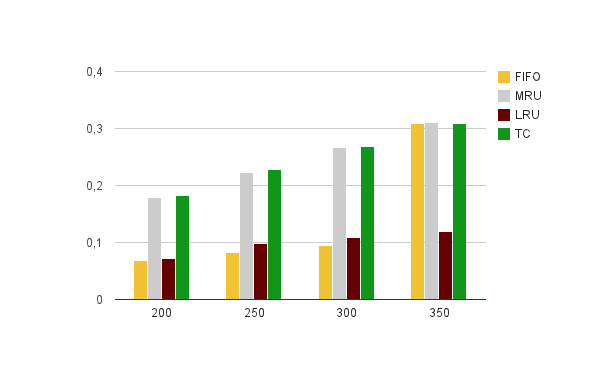
\includegraphics[scale=.80]{grafico1-1}

Random File Scan +File Scan\\
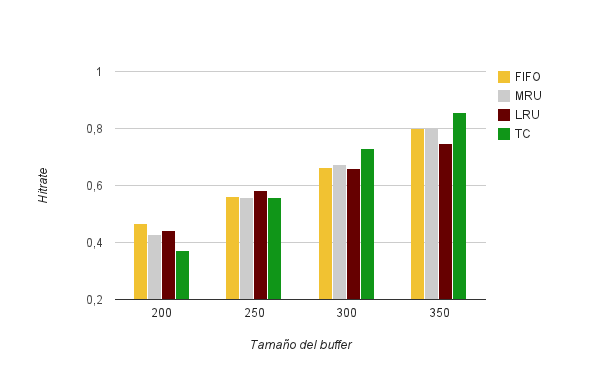
\includegraphics[scale=.80]{grafico1-2}

Random File Sca +Index Scann\\
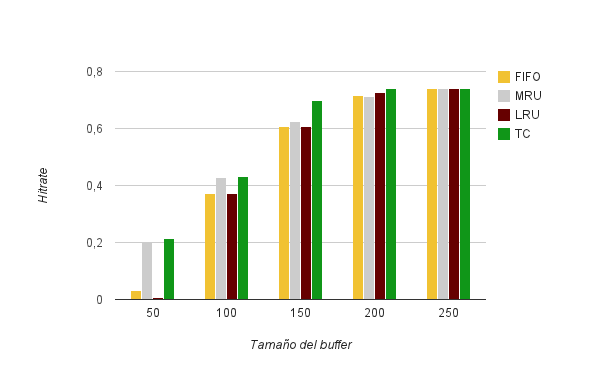
\includegraphics[scale=.80]{grafico2-1}

Mixed Trace +Index Scan\\
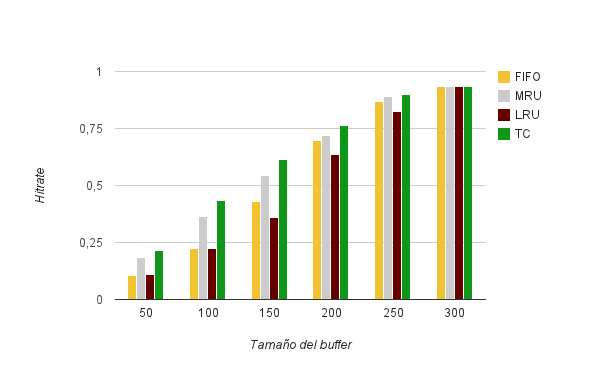
\includegraphics[scale=.80]{grafico2-2}

Mixed Trace only Scan\\
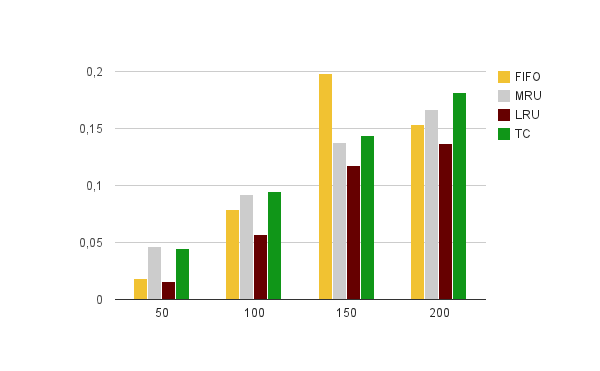
\includegraphics[scale=.80]{grafico3}

\section{Conclusión}

Observando estos gràficos podemos observar que el Touch Count es el que tiene un comportamiento más regular en todos los casos.No obstante siguen existiendo combinaciones de trazas que tendrían un mayor hitrate si se utilizara MRU o LRU. Aunque el Touch Count nos demuestra que abarca una espectro mas amplio de casos podría inducirnos a que quizás siga existiendo espacio para mejorar la selección de
víctimas de un buffer pool. Una posibilidad sería el tratar de que el algoritmo identifique los casos en los que el touchcount no representa la mejor opción antes de aplicarlo.



